\documentclass[letterpaper, 10 pt, conference]{ieeeconf} % letterpaper/a4paper 
% ieeeconf IEEEtran
\IEEEoverridecommandlockouts   % Needed if you want to use the \thanks command
\overrideIEEEmargins

\usepackage[ruled,vlined]{algorithm2e}
\usepackage{amsmath}
\usepackage{amsfonts}
\usepackage{graphicx}

\DeclareMathOperator*{\argmin}{arg\,min}
\DeclareMathOperator*{\argmax}{arg\,max}
\newcommand{\vect}[1]{\mathbf{#1}}
\newcommand{\hvect}[1]{\bar{\vect{#1}}}
\newcommand{\uvect}[1]{\hat{\vect{#1}}}
\newcommand{\field}[1]{\mathbb{#1}}
\newcommand{\Real}[0]{\field{R}}


\title{Modern MAP methods for accurate and faster occupancy grid mapping}
\author{Vikas Dhiman, Brian, Jason J. Corso, Abhijit Kundu, Frank Dallert}
\begin{document}
\maketitle
\begin{abstract}
  Most occupancy grid mapping algorithms have been using two assumption
  algorithm.  \cite{merali2013icra} showed that belief maximization methods
  produce better maps than the traditional two assumption algorithm.  In this
  paper, we show that we can go beyond methods like MCMC Gibbs sampling and
  obtain faster convergence by using modern methods like Sum Product algorithm
  and Dual Decomposition.
\end{abstract}
\section{Problem definition}
A robot equipped with a laser scanner and accurate odometry moves in a static
environment, problem is to figure out an optimal occupancy grid map. For the
purpose of ground robots often 2D maps are enough for path planning and
exploration. 
\section{Two assumption algorithm}
\section{Dropping the assumption}
\section{Representation as factor graph and Notation}
\label{sec:notation}
The problem of Occupancy grid mapping can be expressed as energy minimization
over a factor graph. Let all cells in the map be the variable nodes $V$ and all
the laser measurements be factor nodes $F$. 
There
exists an undirected edge $(i, f)$, if and only if the laser
measurement $f \in F$ passes through the cell $i \in V$. Let $E$ be set of all such edges:
% Mathematically,
\begin{align}
  E = \{(i, f) : i \in V, f \in F, \text{laser $f$ passes through cell $i$}\}
\end{align}
This defines our factor graph representation of occupancy grid mapping $G = (V, F, E)$.

%Let $n(.)$ denote neighborhood in factor graph $G = \{V, F, E\}$.
%
%% unncessary
% i.e
% \begin{align}
%   n(k) &= \begin{cases}
%   \{f \in F: (i, f) \in E\} & \text{ if $k \in V$}\\
%   \{i \in V: (i, f) \in E\} & \text{ if $k \in F$}
%   \end{cases}
% \end{align}
%
Each cell $i \in V$ takes values
from a discrete set of labels $L_i = \{0, 1\}$, where $0$ (respectively $1$) means that
the cell is free (respectively occupied). Also denote the sample space of all the
cells in the map as $\Omega(V) = \prod_{i \in V} L_i$.

Each laser measurement $f \in F$ corresponds to a function $\theta_f : \vect{x}_f \rightarrow \Real$ 
that depends only on the labels of the neighboring cells, $\vect{x}_f = \{x_i\}_{i
\in n(f)}$, and evaluates to an
\emph{energy} value. Here $n(.)$ denotes the neighborhood in the factor graph $G$.
The \emph{energy} can be thought as the negative log likelihood of the given
state $\vect{x}_f$ being the correct state according to the laser measurement $f$.

In this formulation, we seek to determine the label of all the map cells that
maximizes the total likelihood across all measurement, which is equivalent to
minimizing the total \emph{energy} over all factors.
\begin{align}
  \vect{x} = \argmin_{\vect{x} \in \Omega(V)} \sum_{f \in F} \theta_f(\vect{x}_f)
\end{align}
\begin{figure}
  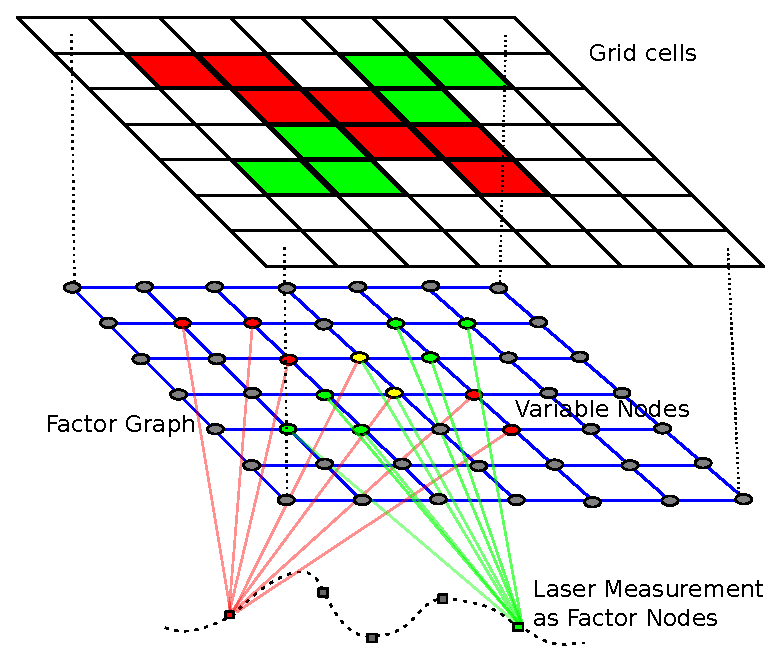
\includegraphics[width=\columnwidth]{../figures/factorgraph/factorgraph.pdf}
  \caption{Diagrammatic conversion of Occupancy Grid to a factor graph.}
  \label{fig:factor-graph}
\end{figure}

\section{Laser sensor model}
\subsection{Gaussian sensor model}
\subsection{Piecewise constant sensor model}
The expected pattern of occupancy from a laser observation is two have last cell as occupied and others as free. So the simplest energy function would be 
\begin{align}
  \theta_f(\vect{x}_f) &= \begin{cases}
              0 & \text{ if } \vect{x}_f = [0, 0 \dots 0, 1]^\top\\
           1000 & \text{ otherwise}
  \end{cases}
\end{align}
where $[0, 0 \dots 0, 1]$ means that all cells are $0$ except the last cell which is $1$. In this context, we consider $\vect{x}^f$ to be a vector of ordered cell labels through which laser measurement $f$ passes.

However, to resolve conflicts it is sometimes better to provide lower energy to all cells free case. Hence, we come with the following energy function.
\begin{align}
  \theta_f(\vect{x}_f) &= \begin{cases}
                     0 & \text{ if } \vect{x}_f = \vect{P}_1\\
                   900 & \text{ if } \vect{x}_f = \vect{P}_2\\
                  1000 & \text{ otherwise}
  \end{cases}
\end{align}
where $\vect{P}_1 = [0, 0 \dots 0, 1]^\top$ and $\vect{P}_2 = [0, 0 \dots 0, 0]^\top$.
\section{Metropolis hastings}
\section2{Heat map}
\section{Sum product}
\cite{kschischang2001factor} introduced the algorithm.
\subsection{Efficient sum product}
\section{Dual decomposition}
\newcommand{\msg}[3]{\mu_{#1#2}(#3)}
\newcommand{\assign}{\leftarrow}
\newcommand{\Sx}{L_i}
Dual decomposition algorithm employs Lagrangian relaxation technique from integer programming to minimize. Here we explain the implementation of the algorithm without going into mathematical derivations. Interested user is referred to \cite{sontag2011introduction,jojic2010accelerated,komodakis2009beyond} for proofs and more variations of the algorithm. 

Pseudo code for Dual decomposition is provided in Alg~\ref{alg:dualdecompostion}. Apart from input factor graph $G = (V, F, E)$ and label set $\{\Sx\}_{i \in V}$ introduced in Sec~\ref{sec:notation}, Dual decomposition depends on a step size $\alpha$.

The idea for Dual decomposition is to split the minimization problem into \emph{slave} problems that can be efficiently minimized. In case of disagreement for minimizing label among slave problems, the messages to slave problems are updated until the slave problems agree with each other. We maintain the minimizing label for variable node $i$, computed by factor $f$ as $x^f_i$.
\begin{algorithm}
  \dontprintsemicolon
  \KwData{\;
  Factor Graph $G = (V, F, E)$\;
  Label set $\{\Sx\}_{i \in V}$\;
  Step size $\alpha > 0$\;
  Maximum number of iterations $N$\;
  }
  \KwResult{Labels $\{x^f_i\}_{(i, f) \in E} $,
  Messages $\{\msg{i}{f}{x_i}\}$}

  $\msg{i}{f}{x_i} \assign 0 \hfill \forall (i, f) \in E, x_i \in \Sx$\;
  $r \assign 1$\;
  \While{$r < N$} {
    \For {$f \in F$} {
      $\vect{x}^f \assign \argmin\limits_{\vect{x}^f} \left( \theta_f(\vect{x}^f) + \sum\limits_{i \in n(f)}\msg{i}{f}{x^f_i} \right)$\;
    }
    \tcc{For disagreeing nodes}
    \For {$i \in V : \exists f, f' \in n(i) : x_i^{f'} \ne x_i^f$} {
      \For{$f \in n(i)$}{
        $\msg{i}{f}{x^f_i} \assign \msg{i}{f}{x^f_i} + \frac{\alpha}{r}$\;
      }
    }
    $r \leftarrow r + 1$\;
  }
  \label{alg:dualdecompostion}
  \caption{Subgradient Dual Decomposition}
\end{algorithm}
We can compute the minimum energy assignment from dual decomposition messages.
\begin{align}
  x_i \assign \argmax\limits_{x_i \in \Sx} \sum\limits_{f \in n(i)} \msg{i}{f}{x_i}
\end{align}
However, the above computation is only valid if the node has at least a pair of disagreeing factors. In case of agreement, we simply take the agreed upon assignment or if the node is not connected to any factors, we take a random assignment.
%%%%%%%%%%%%%%%%%%%%%%%%%%%%%%%% Unncessary
% \begin{algorithm}
%   \dontprintsemicolon
%   \KwData{\;
%     The Variable Node $i \in V$\;
%     Factor Graph $G = (V, F, E)$\;
%     Label set $\Sx$\;
%     Labels $\{x^f_i\}_{f \in n(i)} $\;
%     Messages $\{\msg{i}{f}{x_i}\}$\;
%   }
%   \KwResult{Minimum energy label $x_i$}
%   \tcc{Check for disagreement}
%   \If{$\exists f, f' \in n(i) : x^{f'}_i \ne x^f_i$}{
%     $x_i \assign \argmax\limits_{x_i \in \Sx} \sum\limits_{f \in n(i)} \msg{i}{f}{x_i}$\;
%   } \Else {
%     \tcc{Take any agreed label}
%     $x_i \assign x^f_i : f \in n(i)$\;
%   }
%   \caption{Label from Dual decomposition messages }
%   \label{alg:compute-assignment}
% \end{algorithm}
%%%%%%%%%%%%%%%%%%%%%%%%%%%%%%%% Unncessary
\subsection{Efficient slave minimization of piecewise constant factor}
Minimizing slave problem can be done efficiently for specific kinds of functions, for example, piecewise constant functions.
The problem is to minimize the energy function along with the received messages.
\begin{align}
  \min_{\vect{x}^f} \left( \theta(\vect{x}^f) + \sum_{i \in n(f)}\msg{i}{f}{x^f} \right)
\end{align}
A general minimization algorithm will take time of the order that is exponential in the number of cells a laser passes through as $\vect{x}^f$ can have $|L_i|^{|n(f)|}$ possible values. However, for our sensor model we can make use of the fact that the piecewise function needs to look for only two patterns. We should compute the total function value for these two patterns and the minimum value for the \emph{otherwise} case. 
\begin{align}
    \min \theta_f(\vect{x}_f) = \min &\left( 0 + \sum_{\vect{x}_f = \vect{P}_1, i \in n(f)}\msg{i}{f}{x_i},\right.\\
                            &900 + \sum_{\vect{x}_f = \vect{P}_2, i \in n(f)}\msg{i}{f}{x_i},\\
                            &\left.1000 + \min_{\vect{x}_f \not\in \{\vect{P}_1, \vect{P}_2\}} \sum_{i \in n(f)}\msg{i}{f}{x_i} \right)
\end{align}
The third term can be easily minimized by 
%choosing the minimizing state for each $i$ over all possible $\Omega(\vect{x}_f)$ by 
simply choosing the minimizing $x_i \in L_i$ for each $i$. However, the minimizing labels can coincide with patterns $\vect{P}_1$ and $\vect{P}_2$. The solution is to find minimum three assignments of $\sum_{i \in n(f)}\msg{i}{f}{x_i}$ and pick the one that is not equal to $\vect{P}_1$ nor $\vect{P}_2$. 

%
% Algorithm~\ref{alg:efficient-minimize} gives pseudo code for minimizing the last term.
% \begin{algorithm}
%   \SetKwFunction{ArgSortNElements}{ArgSortNElements}
%   $e_i = \min\limits_{x_i \in L_i} \msg{i}{f}{x_i} \hfill, \forall i \in n(f)$\;
%   $x^*_i = \argmin\limits_{x_i \in L_i} \msg{i}{f}{x_i} \hfill, \forall i \in n(f)$\;
%   $\delta_{if}(x_i) = \msg{i}{f}{x_i} - e_i \hfill, \forall i \in n(f), x_i \in L_i, x_i \ne x^*_i$\;
%   $I = \ArgSortNElements(\delta_{if}(x_i), \lceil{\log_{|L_i|}{3}}\rceil)$\;
%   \caption{Efficient minimization of piecewise constant function}
%   \label{alg:efficient-minimize}
% \end{algorithm}

\subsection{Selection of step size}
Step size is critical choice as it affects the speed with which Dual decomposition converges.
\begin{figure}
  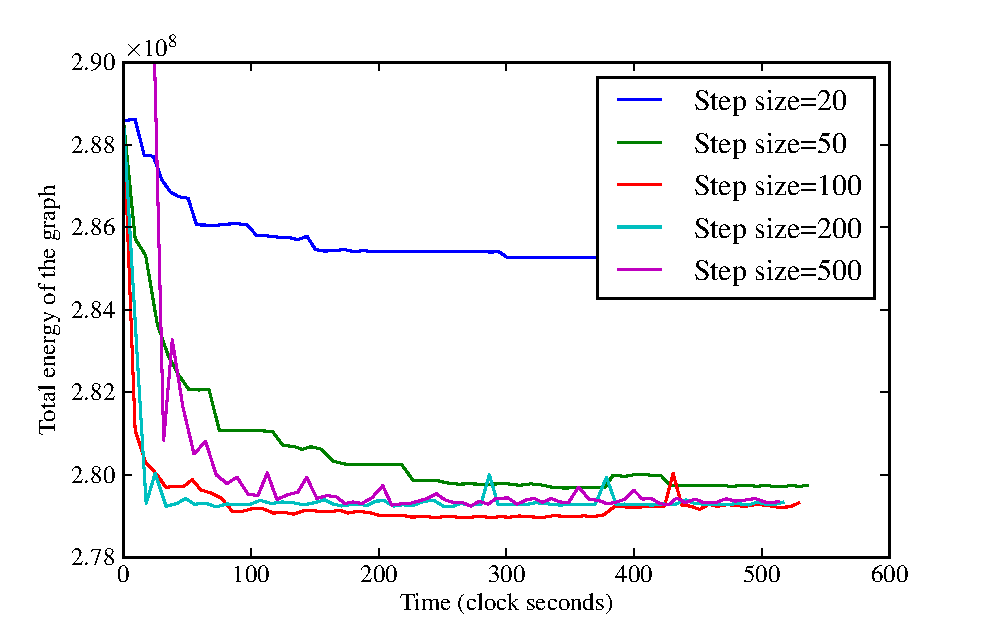
\includegraphics[width=\columnwidth]{../figures/dualdecomposition-stepsize-inc500.pdf}
  \caption{The rate of convergence in dual decomposition depends on step size}
  \label{fig:dualdecomposition-stepsize}
\end{figure}

\section{Experiments} 
Sampling algorithms are liable to getting stuck in a local minima because we flip only one cell at a time.

Dual decomposition converges better because it only focuses on disagreements.

\bibliographystyle{IEEEtran}
\newcommand{\bibdatabase}{/home/vikasdhi/wrk/biblib/bibdb}
\IfFileExists{\bibdatabase.bib}{
  \bibliography{\bibdatabase}
}{
  \bibliography{modern_map}
}
  
\end{document}

